\chapter{Testing}

From the very start of this project, it was planned to observe the \emph{test-driven development (TDD)} convention which suggests to write tests before any logic to define the acceptance criteria of the task. The initially failing but gradually passing tests are then an indicator of progress. Moreover, a perpetual software quality awareness can be achieved when it is coupled with a \emph{continuous integration (CI)} server, which runs the automated tests whenever a change to the source code is pushed to the version control system -- in this case \emph{Git}.

During the progress of this project, this convention turned out to be more difficult than initially thought. Especially in the beginning, when the architecture and interfaces between the various systems, written as part of this project, were not clear yet, writing tests for something which is going to change substantially was counter-productive. It was therefore paused for the sake of progress. However, after achieving a sense of architectural stability, automated tests were completed.

The following sections go into detail for each implemented system.

\section{Integration Framework}

The framework makes extensive use of automated \emph{unit tests}. Unit testing is a software testing method which validates the correctness and executability pieces of software code (\emph{units}) such as functions, methods and classes. In fact, the 39 unit tests provided cover 100 per cent of the source code which means that every line of code is passed during one or more unit tests. The framework utilises \emph{nosetests} to run the tests. Furthermore, the \emph{Software as a Service (SaaS)} and CI platform \emph{Travis CI} is used to build a virtual environment and call nosetests everytime the framework code has been changed. Finally, the SaaS platform \emph{Scrutinizer} is integrated to process the code coverage reports generated by Travis CI. The Travis CI reports can be found here: \url{https://travis-ci.org/halk/recowise}.

First, the unit tests verify that requests to the API routes are accepted and return the correct response. Second, the framework configuration is tested. This goes from validating the XML file against the XML schema defnition as well as verifying that the \texttt{config} object has the correct configuration and resources loaded. Third, the taxonomy logic is tested, in particular the inheritance of taxonomies. Four, the engine adapter base classes, workers as well as the \emph{In-Common} and \emph{Item-Similarity} engine adapters are tested. Notably, it verifies that an event which is subscribed by more than one recommender is notified to all of them. Finally, the \emph{weighted} hybrid engine adapter including its weighting logic is tested. It was important to use \emph{mock objects} which pretend the behaviour of a real object and is helpful to simulate certain edge cases as well as improve the performance of tests. Furthermore, it reduces the chance of chained failures referring to failure which e.g. happens in a low-level function and makes not only the test fail, which tests that function, but all its callers, making troubleshooting difficult.

\section{In-Common Recommender Engine}

This recommender engine has been tested with unit tests covering about 93 per cent of the source code. In fact, the remaining lines are for edge case error handling which could not be simulated. Unit tests are verifying that the API routes, the unserialisation of the request data, parameters such as \texttt{limit} and encoding into JSON are working. Additional unit tests ensure that event data is stored properly and the recommendation query is returning expected recommendations based on events stored. It also validates that a recommendation query is real-time. For example, if a query returns a recommendation and a specific item is removed by an event, then a repetition of this query right after should not contain this recommendation anymore. The unit test in Figure \ref{fig:testing-incommon-recommendation-query} makes sure that a request returns an empty list of recommendations if there are no events happened yet. Finally, data which was created for these tests are removed afterwards. This is to guarantee that the unit tests can be run repeatedly.

\begin{figure}[!ht]
    \begin{minted}{go}
package graph

import (
    "github.com/halk/in-common/model"
    "github.com/stretchr/testify/assert"
    "testing"
)

func TestGetRecommendations_Empty(t *testing.T) {
    rq := model.RecommendationRequest{"Tester", "graphtest4_1", "graphtest4", "tested", 10}
    recommendation, err := GetRecommendations(&rq)
    if err != nil {
        assert.Fail(t, "Unexpected error: "+err.Error())
        return
    }

    assert.IsType(t, model.Recommendation{}, *recommendation, "Unexpected type")
    assert.Len(t, recommendation.Results, 0, "Unexpected length")
}
    \end{minted}
    \caption{In-Common Unit Test Example (Code Listing)}
    \label{fig:testing-incommon-recommendation-query}
\end{figure}

Similar to the framework, Travis CI is used to continuously run tests when changes to the source code are pushed to the repository. The Travis CI reports can be found here: \url{https://travis-ci.org/halk/in-common}.

\section{Item-Similarity Recommender Engine}

The Item-Similarity recommender engine has 4 unit tests with 56 assertions and a code coverage of 94 per cent. Beside validating the API, they are also testing that the similarity algorithm is working as expected (for example comma-separated values, see Figure \ref{fig:test-itemsimilarity-similarity}).

\begin{figure}[!ht]
    \begin{minted}{php}
<?php
namespace Koklu\Tests;

use Silex\WebTestCase;
use Symfony\Component\HttpKernel\Client;

class RecommenderTest extends WebTestCase
{
    // [...]

    public function testCommaSeparatedValues()
    {
        $this->_setCollection('test4');

        $this->_postItem('item1', ['color' => 'red,green', 'size' => 3, 'name' => 'Apple']);
        $this->_postItem('item2', ['color' => 'red', 'size' => 3, 'name' => 'Peach']);
        $this->_postItem('item3', ['color' => 'red', 'size' => 1, 'name' => 'Cherry']);
        $this->_postItem('item4', ['color' => 'green', 'size' => 1, 'name' => 'Grape']);

        $recommendations = $this->_getRecommendation(['item1']);
        $this->assertEquals(
            ['item2' => 0.4, 'item3' => 0.16667, 'item4' => 0.16667], $recommendations
        );
    }

    // [...]
}
    \end{minted}
    \caption{Item-Similarity Unit Test Example (Code Listing)}
    \label{fig:testing-itemsimilarity-similarity}
\end{figure}

The project utilises \emph{PHPUnit} to run the tests. Furthermore, \emph{Travis CI} is used to run the tests everytime a code change has been pushed the source code version control repository. Scrutinizer is integrated to process the code coverage reports generated by Travis CI. The Travis CI reports can be found here: \url{https://travis-ci.org/halk/item-similarity}.

Finally, it was observed that a full export of 189 products from Magento was processed in 100 seconds.

\section{Demo Application Magento}

Although it was planned to have unit tests similar to the framework and recommendation engines as well functional tests, which ensure that the functionality is also working as expected from a user experience perspective, there was no time left to complete it. This was due to the complexity and novelty of Magento2 as well as a lack of documentation on how to run and extend automated tests.

Nonetheless, manual functional tests have been carried out throughout the project lifetime. For the In-Common recommender engine, recommendations were observed by performing user behaviour in two independent browser windows, simulating two customers with similar behaviour pattern (Figure \ref{fig:testing-magento-myaccount}). Then, the data on the user interface of the graph database management system Neo4j.

\begin{figure}[!ht]
    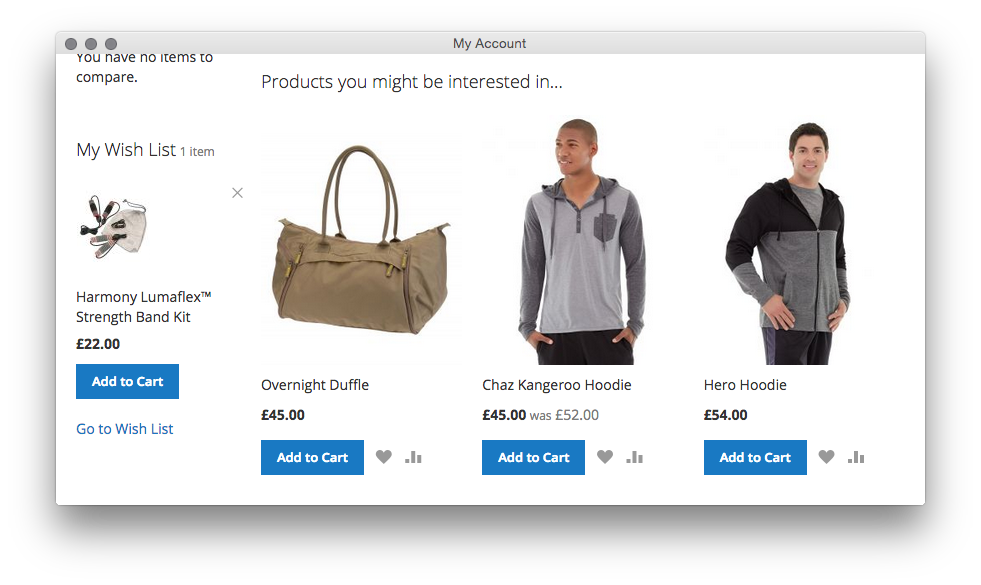
\includegraphics[width=\textwidth,center]{screens/myaccount.png}
    \caption{Recommendations in Customer Account (Screenshot)}
    \label{fig:testing-magento-myaccount}
\end{figure}

For the Item-Similarity recommender engine, a full export has been performed and the MongoDB database reviewed. A full export of 189 products to the framework took 7 seconds on the Vagrant environment. It is performed in batches and can handle far more products. Changes to the product data have been simulated and observed that the recommender engine is processing those properly. Finally, the recommendation quality on the basket page has been reviewed.